\documentclass{article}
\usepackage{geometry}
\usepackage[utf8]{inputenc}
\usepackage{amsmath}
\usepackage{amssymb}
\usepackage{amsfonts}
\usepackage{esint}
\usepackage{indentfirst}
\usepackage{color}   %May be necessary if you want to color links
\usepackage{hyperref}
\newcommand{\cmark}{\ding{51}}%
\newcommand{\xmark}{\ding{55}}%
\usepackage{tikz}
\newcommand{\Plus}{\mathord{\begin{tikzpicture}[baseline=0ex, line width=1, scale=0.13]
\draw (1,0) -- (1,2);
\draw (0,1) -- (2,1);
\end{tikzpicture}}}
\newcommand\Tau{\mathcal{T}}
\usepackage{bbm}
\newcommand{\indep}{\rotatebox[origin=c]{90}{$\models$}}

\usepackage{authblk}
\usepackage[natbib, maxbibnames=5, sorting=none]{biblatex}
\addbibresource{references.bib} 

\graphicspath{ {./figures/} }
\usepackage{subcaption} 

\hypersetup{
    colorlinks=true, %set true if you want colored links
    linktoc=all,     %set to all if you want both sections and subsections linked
    linkcolor=blue,  %choose some color if you want links to stand out
}
%\usepackage{geometry}
%\geometry{a4paper,scale=0.7}

\title{Leveraging noisy qualitative data for effective parameter inference in biophysical models}
\date{}
\author[1,2]{Jinghao Chen\thanks{chen.jinghao.3n@kyoto-u.ac.jp, jinghc2@uci.edu}}
\author[3]{William S. Hlavacek\thanks{wish@lanl.gov}}
\date{}
\affil[1]{\small Institute for the Advanced Study of Human Biology, Kyoto University, Japan}
\affil[2]{Department of Mathematics, University of California, Irvine, USA}
\affil[3]{Theoretical Division, Los Alamos National Laboratory, USA}

\begin{document}

\maketitle

\begin{abstract}
    Current mathematical models often emphasize high-precision quantitative data, overlooking the potential of noisy qualitative data, which is frequently generated in biological experiments but underutilized in modeling efforts. In this study, we reanalyzed DNA sequences from massively parallel experiments that characterize gene expression levels, encountering noisy data grouped into finite categories. To further address the challenges in the resolution of the data, only a subset of such data was selected and was further downscaled into 2-bin binary classes intentionally. Despite this deliberate simplification, the detailed protein-DNA binding energy distribution was successfully reconstructed through parameterizing the biological model using a straightforward negative logistic likelihood with stochastic gradient descent. Uncertainty quantification was performed using bootstraps. Our approach demonstrated consistency with outcomes from more complex models using refined data, precisely matching all known consensus sequences. Furthermore, other crucial parameters were jointly inferred, some of which were previously unattainable through existing models. We also introduced alternative parameterization methods, including a hinge loss function with a soft margin penalty and an extension of the negative logistic loss into a multi-category scenario, both replicating similar results. This research highlights the potential of noisy qualitative biological data and demonstrates that, with appropriate model parameterization approaches, we can extract meaningful insights into the underlying mechanisms of gene expression regulation.
\end{abstract}

\newpage
\tableofcontents

\newpage
\section{Introduction}

In the current landscape of mathematical modeling, there is a predominant focus on high-precision quantitative data, often overlooking the inherent noise and complexity of biological data. Our research, however, seeks to address this gap by leveraging high-throughput, low-resolution qualitative data for the parameterization of biological models, with promising results.

Our primary emphasis lies in the parameterization of a biophysical model, detailed in Appendix Section \ref{sup sec: tau model} Eq. \ref{eq: tau model}, pertaining to the regulation of the lac operon in E. coli, which was originally presented by Kuhlman \textit{et al.} \cite{Kuhlman2007PNAS}. To achieve this, we undertook a reanalysis of high-throughput transcription regulatory sequences (TRS) data, as generated by Kinney \textit{et al.} \cite{Kinney2010PNAS}. It is worth noting that Kinney \textit{et al.} had previously performed model parameter inference using a method based on mutual information. However, this method had inherent limitations, particularly in its inability to infer certain model parameters. Moreover, it relied on an artificial "pseudo likelihood," rendering it statistically unreliable for uncertainty quantification.

Our research endeavor aims to surmount these limitations and, in the process, demonstrate the efficacy of inferring model parameters from low-quality datasets characterized by less data and lower resolution.

The primary objectives of this project encompass the following:

\begin{itemize}
\item Reanalysis of DNA sequence data originally presented by Kinney \textit{et al.} \cite{Kinney2010PNAS}. This involves downsampling the data into binary labels linked to only two fluorescence levels.
\item Parameterization of the biophysical model initially proposed by Kuhlman \textit{et al.} \cite{Kuhlman2007PNAS}. This parameterization is achieved using statistically interpretable techniques, such as negative logistic likelihood. This approach is adopted to address the limitations observed in the mutual information method employed by Kinney \textit{et al.} \cite{Kinney2010PNAS}.
\item The development of alternative parameterization methods and the extension of existing approaches from binary classifiers to more versatile and robust multi-category classifiers.
\item A comprehensive assessment of the results and the implementation of uncertainty quantification through bootstrapping.
\end{itemize}

\section{Model parameterization}

\subsection{Data processing}\label{sec: downsampling}

We have a dataset consisting of $M_0$ sequences, denoted as $\{\sigma_k\}_{k=1}^{M_0}$, along with their corresponding fluorescence levels, denoted as $\{\mu_k\}_{k=1}^{M_0}$. This dataset combines batches from 1 to 9, where for any $k=1,2,...,M_0$:

\begin{equation}\label{eq: 9 flurescence}
    \mu_k \in \{1,2,3,4,5,6,7,8,9\}
\end{equation}

To simplify the fluorescence levels, we use the bin-5 fluorescence as the reference level. By dropping bin-5 data, we can represent the fluorescence levels as binary classes, denoted as $\{y_k\}_{k=1}^M$:

\begin{equation}\label{eq: binary fluorescence}
\begin{aligned}
y_k=\left\{
\begin{aligned}
& 1 &,\mu_k > 5 \\
& 0 &,\mu_k < 5
\end{aligned}
\right.
\end{aligned}
\end{equation}

\noindent which is a reduced dataset, where the bin-5 category has been excluded. The data resolution has been minimized, with the transition from 9 classes in Eq. \ref{eq: 9 flurescence} to binary in Eq. \ref{eq: binary fluorescence} (the lowest possible resolution).

\subsection{Negative logistic likelihood}

Let $\bar{\tau}$ be the reference rate of transcription associate with bin-5 fluorescence level. Hence,

\begin{equation}
\begin{aligned}
\left\{
\begin{aligned}
& \tau_\theta (\sigma_k) > \bar{\tau}, \;\text{ if } y_k = 1 \\
& \tau_\theta (\sigma_k) < \bar{\tau}, \;\text{ if } y_k =0 
\end{aligned}
\right.\;\;\;\text{for } k = 1, 2, ..., M 
\end{aligned}
\end{equation}

Now we can construct the negative logistic likelihood (NLL) loss:

\begin{equation}\label{eq: nll loss for tau}
    J = -\frac{1}{M}\sum_{k=1}^M [y_k\cdot\log(S(\tau_k-\bar{\tau}))+(1-y_k)\cdot\log(1-S(\tau_k-\bar{\tau}))],
\end{equation}

\noindent where $S$ is the standard sigmoid function

\begin{equation}
    S(x)=\frac{1}{1+e^{-x}}.
\end{equation}

For the model of rate of transcription please see Appendix Section \ref{sup sec: tau model} Eq. \ref{sup sec: tau model}. The binding energies of CRP and RNAP are assumed to be the sum of energies through all the binding positions, detailed in Appendix Section \ref{sup sec: energy matrix model}. It is important to note that $\tau_k$ contains a scaling factor $\tau_{\text{max}}$, making it challenging to directly infer the exact values of both the maximal transcription rate $\tau_{\text{max}}$ and reference transcription rate $\bar{\tau}$. Nevertheless, we can deduce their ratio $\bar{\tau}/\tau_{\text{max}}$ by applying

\begin{equation}
    \frac{\tau_k-\bar{\tau}}{\tau_{\text{max}}} = \frac{C_r e^{-\varepsilon_r/RT}+C_c C_r e^{-(\varepsilon_c+\varepsilon_r+\varepsilon_i)/RT}}{1+C_c e^{-\varepsilon_c/RT}+C_r e^{-\varepsilon_r/RT}+C_c C_r e^{-(\varepsilon_c+\varepsilon_r+\varepsilon_i)/RT}} - \frac{\bar{\tau}}{\tau_{\text{max}}}
\end{equation}

\noindent in the loss functions (Eq. \ref{eq: nll loss for tau}). Hence, we aim to infer a set of parameters denoted as:

\begin{equation}
\hat{\theta} = \left(\frac{\bar{\tau}}{\tau_{\text{max}}},C_c,C_r,\varepsilon_i,[\text{CRP energy matrix}],[\text{RNAP energy matrix}]\right)
\end{equation}

\noindent where these parameters are obtained by minimizing the loss function:

\begin{equation}\label{eq: optimization problem}
\hat{\theta}=\arg\min_\theta J.
\end{equation}


\subsection{Alternative model: hinge loss with soft margin}\label{sec: hinge loss model}

\begin{figure}[htbp]
\centering
\begin{subfigure}{.45\textwidth}
  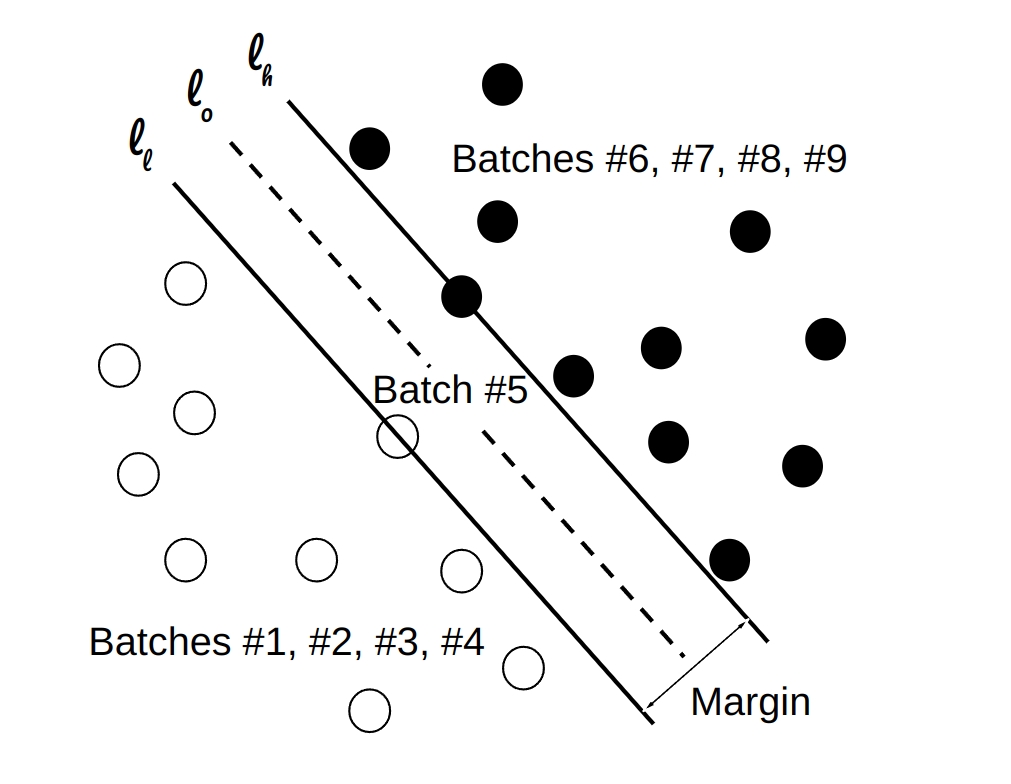
\includegraphics[width=1\linewidth]{figures/230803_svm_demo.png}
  \caption{Margin.}
  \label{fig: svm graph demo}
\end{subfigure}
\begin{subfigure}{.45\textwidth}
  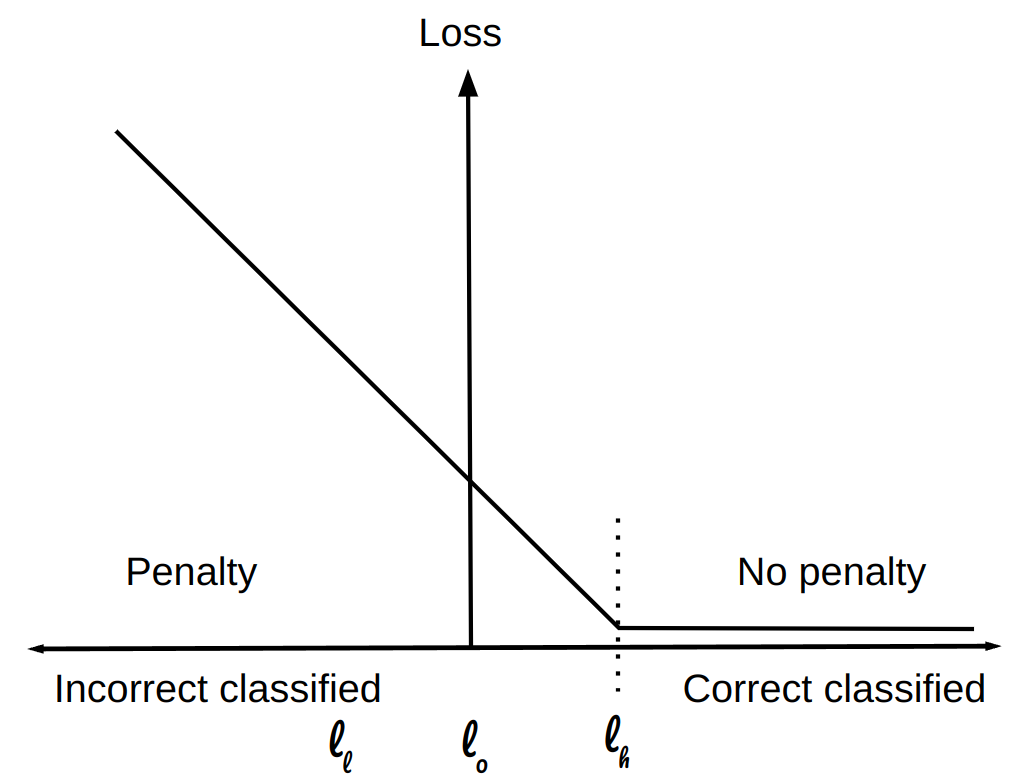
\includegraphics[width=1\linewidth]{figures/230803_hinge_function.png}
  \caption{Hinge.}
  \label{fig: hinge function}
\end{subfigure}
\caption{An alternative model based on Support Vector Machine (SVM).}
\label{fig: svm}
\end{figure}

We now aim to incorporate the static penalty introduced by Mitra \textit{et al.} \cite{Mitra2018NatCommun} to devise a more straightforward yet equally effective loss function. Since the entire bin-5 has been dropped, it is natural to consider a margin separating two classes of data instead of just a single layer hyperplane (Fig. \ref{fig: svm graph demo}). That is, for the class labeled by $y_k=1$, 

\begin{equation}
    \exists \Delta\tau>0 \;\; \text{s.t.} \;\; \tau_k >\bar{\tau}+\Delta\tau
\end{equation}

\noindent and $\tau_k<\bar{\tau}-\Delta\tau$ for the class labeled as $y_k=0$. Without loss of generality, these non-dimensional rate of transcription can be rescaled to yield a unit $\Delta\tau=1$, hence the hinge loss can be formulated from static penalties accordingly:

\begin{equation}\label{eq: hinge loss for tau}
    J = \frac{1}{M}\sum_{k=1}^M \max{(0,1+(2y_k-1)\cdot(\tau_k-\bar{\tau}))}.
\end{equation}

When $y_k=0$, the linear penalty is applied as $\tau_k$ exceeds $\bar{\tau}-1$, and its magnitude is proportional to the amount by which it surpasses this threshold. Similarly, when $y_k=1$, the linear penalty is applied as $\tau_k$ falls below $\bar{\tau}+1$, and its magnitude is proportional to the deviation from this bound (Fig. \ref{fig: hinge function}). This implies that the range $[\bar{\tau}-1,\bar{\tau}+1]$ represents the (non-dimensional) reference rate of transcription span for bin-5 sequences.

The hinge loss defined in Eq. \ref{eq: hinge loss for tau} serves as a soft margin support vector machine (SVM) model, effectively penalizing misclassifications. This insight prompts us to explore the margin width, which can be quantitatively expressed as a function of the energy matrix:

\begin{equation}
    \frac{2}{\|(\tau_k)_{k=1}^M\|}
\end{equation}

\noindent where $\|\cdot\|$ takes the $L^2$ norm

\begin{equation}
    \|(\tau_k)_{k=1}^M\| = \sqrt{\sum_{k=1}^M \tau_k^2}.
\end{equation}

\subsection{Model extension: multi-category scenario}

In contrast to binary classification ($y_k=0$ or $1$), our model is being extended to a multi-category scenario. In binary classification, the probability of a fluorescence level being higher than the reference level ($y_k=1$) conditioned on the sequence-based parameter $\theta$ can be interpreted as the cumulative probability function of parameter $\theta$ \cite{Mitra2018NatCommun}. In other words,

\begin{equation}
\mathbbm{P}(y_k=1|\theta) = \mathbbm{P}(\tau_k>\bar{\tau}|\theta) = cdf(\theta,\sigma_k,\bar{\tau})=S(\tau_\theta(\sigma_k)-\bar{\tau}),
\end{equation}

\noindent while conversely,

\begin{equation}
\mathbbm{P}(y_k=0|\theta) = 1-\mathbbm{P}(y_k=1|\theta).
\end{equation}

Analogously, we can define conditional probabilities for the multi-category case. Instead of a single threshold $\bar{\tau}$, we now require two thresholds, $\bar{\tau}_1$ and $\bar{\tau}_2$, for three classes:

\begin{equation}
\begin{aligned}
    \mathbbm{P}(\tau_k<\bar{\tau}_1|\theta) &= 1-cdf(\theta,\sigma_k,\bar{\tau}_1) \\
    \mathbbm{P}(\bar{\tau}_1<\tau_k<\bar{\tau}_2|\theta) &= cdf(\theta,\sigma_k,\bar{\tau}_1) - cdf(\theta,\sigma_k,\bar{\tau}_2)\\
    \mathbbm{P}(\tau_k>\bar{\tau}_2|\theta) &= cdf(\theta,\sigma_k,\bar{\tau}_2)
\end{aligned}
\end{equation}

Assuming that $\bar{\tau}_1$ and $\bar{\tau}_2$ are sufficiently separated, we can simplify the probability $\mathbbm{P}(\bar{\tau}_1<\tau_k<\bar{\tau}_2|\theta)$ as follows:

\begin{equation}
\mathbbm{P}(\bar{\tau}_1<\tau_k<\bar{\tau}_2|\theta) = cdf(\theta,\sigma_k,\bar{\tau}_1)(1- cdf(\theta,\sigma_k,\bar{\tau}_2))
\end{equation}

Consequently, the loss function for the multi-category scenario can be expressed as:

\begin{equation}
J = -\frac{1}{M}\sum_{k=1}^M \sum_{i=1}^2 [y_k\cdot\log(S(\tau_\theta(\sigma_k)-\bar{\tau}_i))+(1-y_k)\cdot\log(1-S(\tau\theta(\sigma_k)-\bar{\tau}_i))]
\end{equation}

This loss function accommodates multiple categories for an improved understanding of the data.


\section{Results}

Due to the large size of our dataset, we employed the stochastic gradient descent method with 500 epochs to search for the optimal energy matrices (Fig. \ref{fig: energy matrices}). Other model parameters in the biophysical model (Eq. \ref{eq: tau model}) can be jointly inferred with energy matrices. To assess the degree of uncertainty, we executed bootstrapping, with the outcomes illustrated in Fig. \ref{fig: bootstrapping}.

\begin{figure}[htbp]
\centering
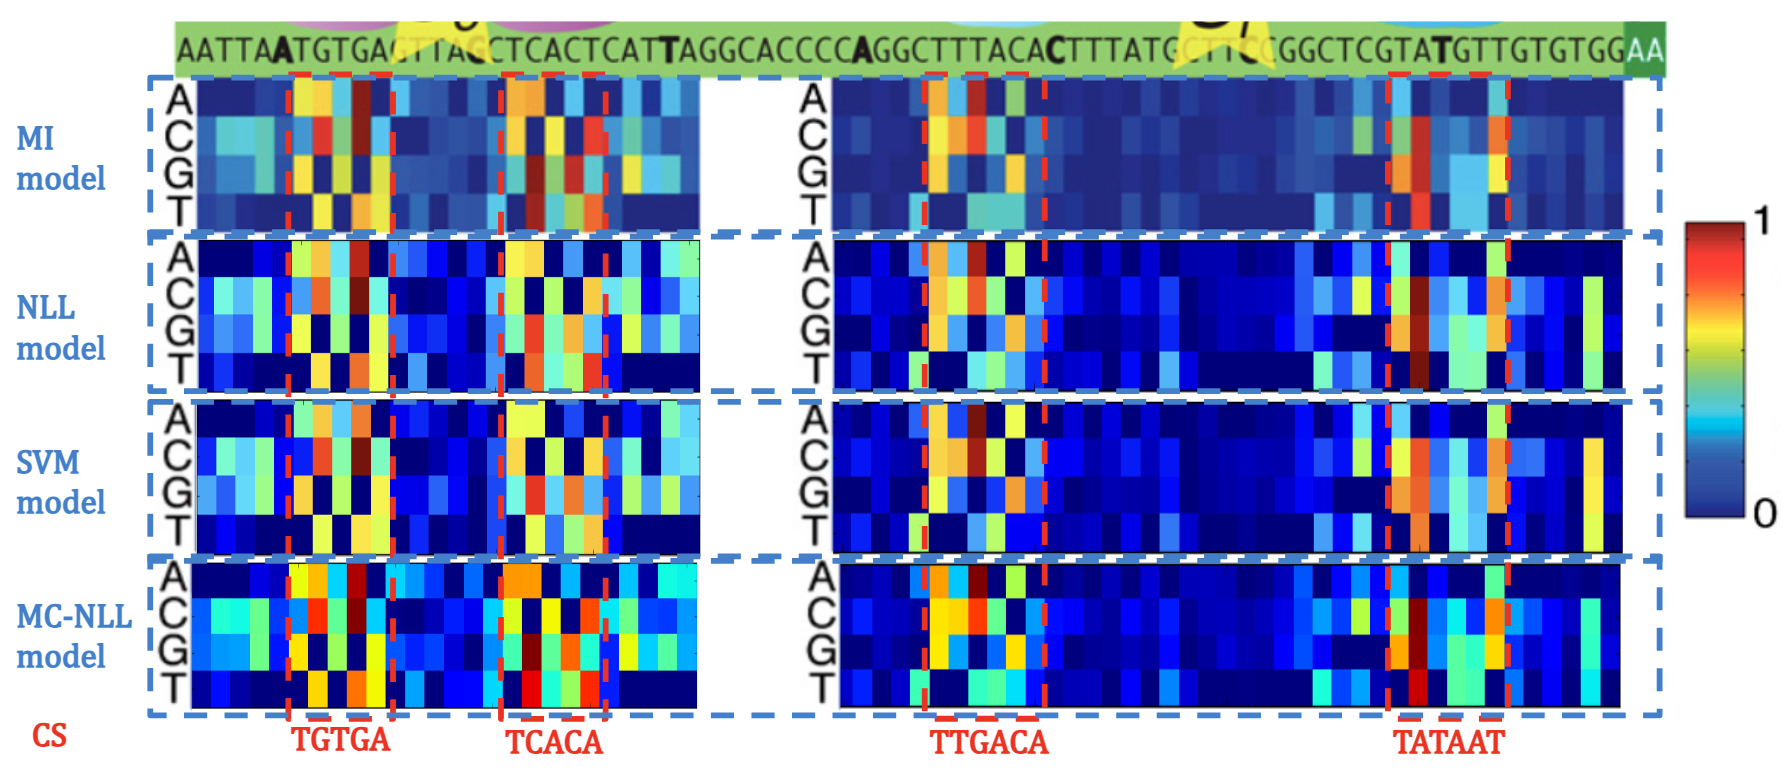
\includegraphics[width=1\linewidth]{figures/230908_energy_matrices.png}
\caption{Energy matrices trained using various models. From top to bottom: MI model by Kinney \textit{et al.} \cite{Kinney2010PNAS} based on mutual information; NLL model and SVM model as binary classifiers developed in our study, and MC-NLL model representing the multi-category NLL model introduced in the model extension section. Consensus sequences (CS) are highlighted in red at the bottom, corresponding to entries with the lowest binding energy (shown in the darkest blue color) for each position in the energy matrices.}
\label{fig: energy matrices}
\end{figure}

\begin{figure}[htbp]
\centering
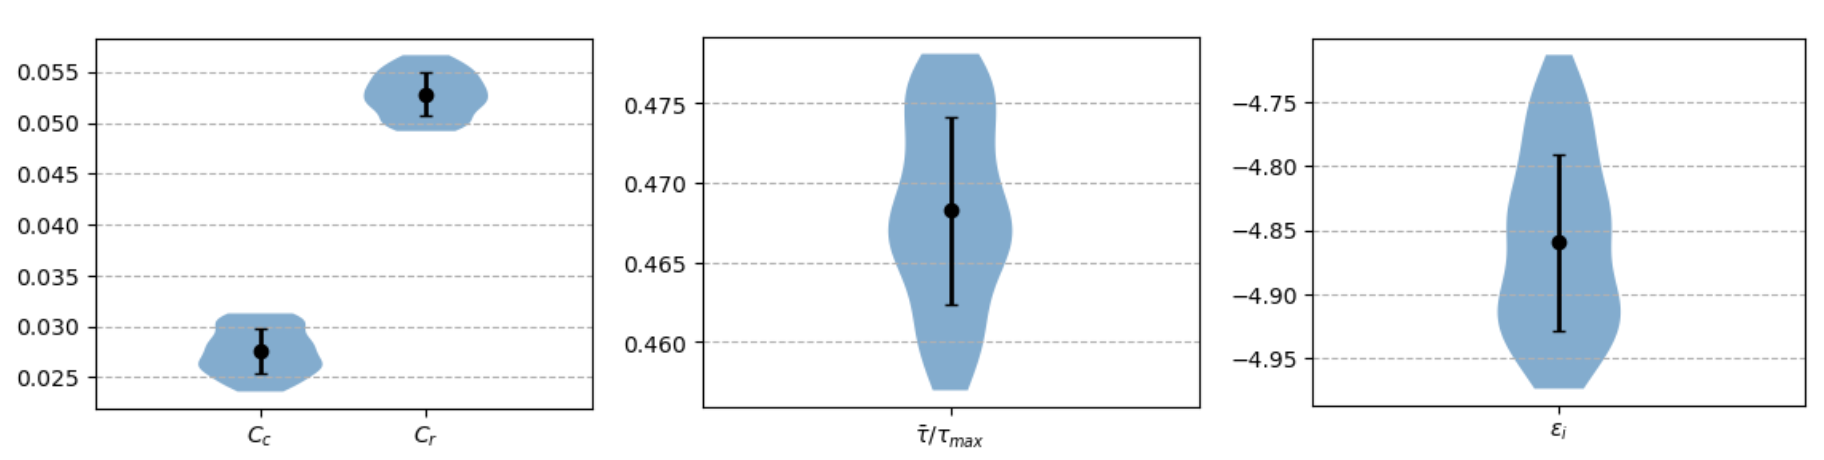
\includegraphics[width=1\linewidth]{figures/230908_bootstrapping.png}
\caption{Bootstrapping results.}
\label{fig: bootstrapping}
\end{figure}

In Table \ref{table: model params}, we present a comparative analysis of our results with those of Kinney \textit{et al.} This table highlights our ability not just to replicate the energy matrices (see Fig. \ref{fig: energy matrices}) but also to derive crucial model parameters, notably $C_r$ and $\bar{\tau}/\tau_{\text{max}}$. It is worth noting that these parameters were proved to be unattainable using mutual information approach \cite{Kinney2010PNAS}.

\begin{table}[htbp]
    \centering
\begin{tabular}{ | c c c | }
\hline
 model parameter & J Kinney \textit{et al.} 2010 & J Chen \textit{et al.} 2023\\ 
 \hline
 \hline
 $\bar{\tau}/\tau_{\text{max}}$ & unknown & $0.467 \pm 0.005$ \\
 $C_c$  & $10^{-1.2\pm 0.2}$ & $0.027\pm 0.002$\\
 $C_r$  & unknown & $0.053\pm 0.002$\\
 $\varepsilon_i$ &  $-3.26\pm 0.41$ \text{ kcal/mol} & $-4.855\pm 0.077$ \text{ kcal/mol}\\
 \hline
\end{tabular}
    \caption{Inferred parameters for normalized reference transcription rate $\bar{\tau}/\tau_{\text{max}}$, CRP concentration $C_c$, RNAP concentration $C_r$ and CRP-RNAP interaction energy $\varepsilon_i$.}
    \label{table: model params}
\end{table}

Finally, we can assess the accuracy of our binary classifier, as shown in Figure \ref{fig: accuracy}. In this example, we use the NLL model, and similar observations apply to the SVM model. It's noteworthy that accuracy is relatively higher when the data is far from the threshold (bin-5), which is to be expected. Overall, the accuracies across the batches are consistently high.

\begin{figure}[htbp]
\centering
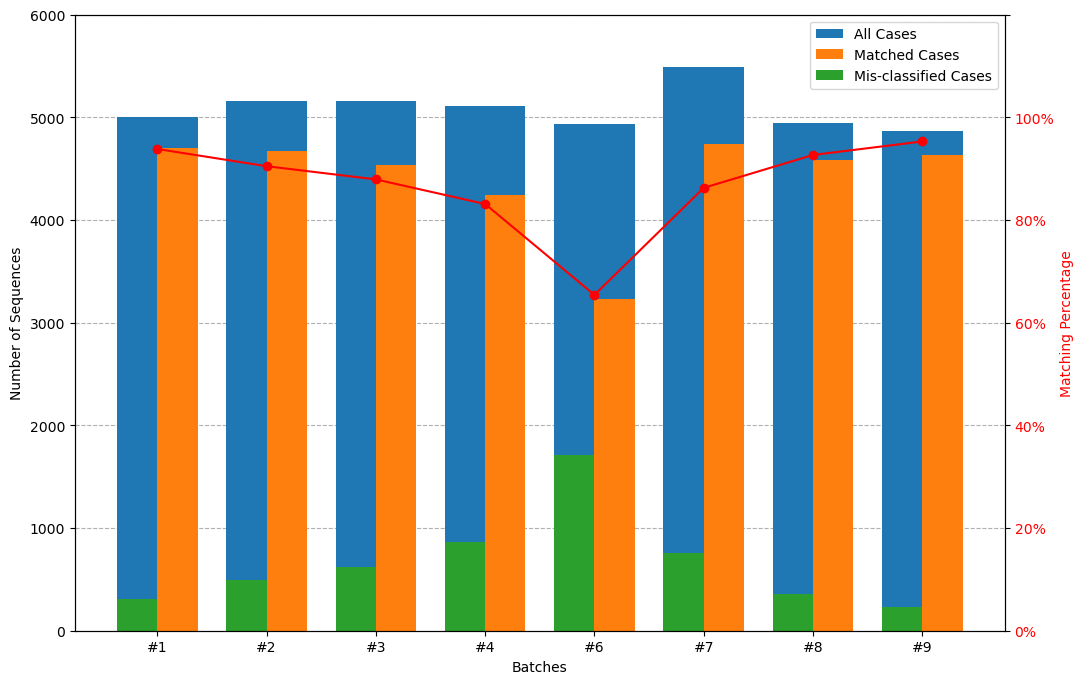
\includegraphics[width=.8\linewidth]{figures/2300908_accuracy.png}
\caption{Accuracy quantification.}
\label{fig: accuracy}
\end{figure}


\section{Discussion}


\section{Acknowledgement}

This research was supported in part by an appointment with the National Science Foundation (NSF) Mathematical Sciences Graduate Internship (MSGI) Program. This program is administered by the Oak Ridge Institute for Science and Education (ORISE) through an interagency agreement between the U.S. Department of Energy (DOE) and NSF. ORISE is managed for DOE by ORAU. All opinions expressed in this paper are the author's and do not necessarily reflect the policies and views of NSF, ORAU/ORISE, or DOE.


\newpage
\printbibliography


\newpage
\section{Appendix}

\subsection{Model of transcription rate}\label{sup sec: tau model}

In accordance with Kuhlman \textit{et al.} \cite{Kuhlman2007PNAS}, we made an assumption that the transcription rate $\tau$ at the \textit{lac} promoter is directly related to the presence of RNA polymerase (RNAP) at its binding site in a state of thermal equilibrium. This relationship is quantitatively described as follows:

\begin{equation}\label{eq: tau model}
    \tau = \tau_{\text{max}}\frac{C_r e^{-\varepsilon_r/RT}+C_c C_r e^{-(\varepsilon_c+\varepsilon_r+\varepsilon_i)/RT}}{1+C_c e^{-\varepsilon_c/RT}+C_r e^{-\varepsilon_r/RT}+C_c C_r e^{-(\varepsilon_c+\varepsilon_r+\varepsilon_i)/RT}}.
\end{equation}

The model given above involves several parameters: $\tau_{\text{max}}$, the transcription rate with full RNAP occupancy; $C_c$ and $C_r$, the concentrations of CRP and RNAP; $R=1.98\times 10^{-3} \;\text{kcal/mol}^\circ\text{K}$, the gas constant; and $T=310^\circ\text{K}$, the cell-induced temperature. The key parameter is $\varepsilon_i$, representing the interaction energy between CRP and RNAP. In short, these model parameters can be summarized in the following Table \ref{table: model params list}.

\begin{table}[htbp]
    \centering
\begin{tabular}{ | c c | }
\hline
 model parameter & meaning\\ 
 \hline
 \hline
 $\varepsilon_c$ & CRP binding energy \\
 $\varepsilon_r$ & RNAP binding energy \\
 $\varepsilon_i$ & CRP-RNAP interaction energy  \\
 $C_c$ & CRP concentration \\
 $C_r$ & RNAP concentration \\
 $\tau_{\text{max}}$ & maximal transcription rate \\
 $R$ & gas constant ($1.98\times 10^{-3} \;\text{kcal/mol}^\circ\text{K}$)\\ 
 $T$ & cell-induced temperature ($310^\circ\text{K}$)\\
 \hline
\end{tabular}
    \caption{Model parameters for Eq. \ref{eq: tau model}.}
    \label{table: model params list}
\end{table}

It is noteworthy that $\varepsilon_c$ and $\varepsilon_r$ are the only sequence-dependent parameters in this model, while all other parameters remain constant for different sequence inputs $\sigma_k$. Importantly, the transcription rate $\tau$ exhibits global monotonicity (monotonic increasing) with respect to both $\varepsilon_c$ and $\varepsilon_r$. Hence, we can write the transcription rate of sequence $\sigma_k$ as $\tau_k:=\tau(\epsilon_{c,k},\epsilon_{r,k})=\tau(\sigma_k)$, and set the reference transcription rate $\bar{\tau}$ to be the transcription rate of sequences in bin-5.


\subsection{Energy matrix}\label{sup sec: energy matrix model}

Recall that the energy matrix models: each base within a protein’s binding site was assumed to contribute additively to the overall binding energy \cite{Kinney2010PNAS}. Under this hypothesis, the binding energy of CRP $\varepsilon_c$ can be decomposed as

\begin{equation}\label{eq: energy matrix}
    \varepsilon_c = \sum_{i=-74}^{-49} \varepsilon_c^{i}
\end{equation}

\noindent where $\varepsilon_c^{i}$ is the binding energy at the position $i$, which depends on the nucleotide $b$ at position $i$:

\begin{equation}\label{eq: energy at site i}
    \varepsilon_c^{i} (b) 
    = \varepsilon_c^{i,A} \cdot \mathbbm{1}_A(b)+\varepsilon_c^{i,C} \cdot \mathbbm{1}_C(b)+\varepsilon_c^{i,G} \cdot \mathbbm{1}_G(b)+\varepsilon_c^{i,T} \cdot \mathbbm{1}_T(b)
\end{equation}

Here, $\mathbbm{1}_A(b)$ is the indicator function (characteristic function) defined as 

\begin{equation}
\begin{aligned}
\mathbbm{1}_A(b)=\left\{
\begin{aligned}
& 1 &,b=A \\
& 0 &,\text{otherwise}
\end{aligned}
\right.
\end{aligned}
\end{equation}

\noindent and analogously for $\mathbbm{1}_C(b)$, $\mathbbm{1}_G(b)$ and $\mathbbm{1}_T(b)$.

By collecting the energy weights $\varepsilon_c^{i,b}$ for all possible bases $b\in\{A,C,G,T\}$ and binding positions $i\in [-74,-49]\cap\mathbb{Z}$, we can construct the energy matrix of CRP, denoted as $\theta_c=(\varepsilon_c^{i,b})$, which has 4 rows and 26 columns. Now, the total binding energy of CRP on a sequence $\sigma=(b_i)_{i=-74}^{-49}$ in Eq. \ref{eq: energy matrix} can be rewritten as

\begin{equation}\label{eq: energy matrix function}
    \varepsilon_c(\sigma) = \sum_{i=-74}^{-49} \varepsilon_c^{i}(b_i).
\end{equation}

\subsection{Energy shift}\label{sup sec: energy shift}

The energy matrices have been adjusted for convention. Following the energy matrix model assumption, where each \textit{lac} promoter site contributes independently and additively to the total binding energy, we set the minimal entry at each individual column to 0, representing the wild-type \textit{lac} promoter site having zero energy. Furthermore, the results obtained from the model are non-dimensional, allowing us to rescale the values to a range between 0 and 1 by dividing each entry by the maximal value in the entire matrix. This rescaling is convenient since the dimensional matrix is determined only up to a multiplicative constant, and it ensures that the energy matrix remains comparable and interpretable across different experiments or datasets. 

After obtaining the dimensional energy matrix, we can calculate the energy shift in units of kcal per mol by summing up all the individual shifting amounts at each site. According to Kinney \textit{et al.} \cite{Kinney2010PNAS}, this energy shift is approximately -7 kcal/mol for CRP and around -8.3 kcal/mol for RNAP.

Let's assume that at site $i$, the energy shift is represented by $\delta_i$ (to avoid abusing the notation since $\varepsilon_i$ is the interaction energy between CRP and RNAP), and the binding energy is denoted as $\hat{\varepsilon}^i_c (b)$. As a reference, the binding energy at position $i$ without energy shifting, denoted by $\varepsilon_c^{i} (b)$, is shown in Eq. \ref{eq: energy at site i}. Now, the modified $\hat{\varepsilon}^i_c (b)$ can be expressed in the following form:

\begin{equation}\label{eq: shift and no shift detailed}
\begin{aligned}
    \hat{\varepsilon}_c^{i} (b) 
    = & (\varepsilon_c^{i,A}+\delta_i) \cdot \mathbbm{1}_A(b)
    +(\varepsilon_c^{i,C}+\delta_i) \cdot \mathbbm{1}_C(b) \\
    &+(\varepsilon_c^{i,G}+\delta_i) \cdot \mathbbm{1}_G(b)
    +(\varepsilon_c^{i,T}+\delta_i) \cdot \mathbbm{1}_T(b) \\
    =& \varepsilon_c^{i,A} \cdot \mathbbm{1}_A(b)+\varepsilon_c^{i,C} \cdot \mathbbm{1}_C(b)+\varepsilon_c^{i,G} \cdot \mathbbm{1}_G(b)+\varepsilon_c^{i,T} \cdot \mathbbm{1}_T(b) \\
    &+ \delta_i \cdot (\mathbbm{1}_A(b)+\mathbbm{1}_C(b)+\mathbbm{1}_G(b)+\mathbbm{1}_T(b)) \\
    =& \varepsilon_c^{i} (b) + \delta_i \cdot (\mathbbm{1}_A(b)+\mathbbm{1}_C(b)+\mathbbm{1}_G(b)+\mathbbm{1}_T(b)).
\end{aligned}
\end{equation}

Since $b\in \{A,C,G,T\}$, we have

\begin{equation}  \mathbbm{1}_A(b)+\mathbbm{1}_C(b)+\mathbbm{1}_G(b)+\mathbbm{1}_T(b)\equiv 1,
\end{equation}

\noindent therefore Eq. \ref{eq: shift and no shift detailed} goes to

\begin{equation}\label{eq: energy at site i with shift}
    \hat{\varepsilon}_c^{i} (b) = \varepsilon_c^{i} (b) + \delta_i.
\end{equation}

Now with Eq. \ref{eq: energy at site i with shift}, the total binding energy of CRP (the form without energy shifting is Eq. \ref{eq: energy matrix function}) becomes

\begin{equation}
\begin{aligned}
    \hat{\varepsilon}_c(\sigma) &= \sum_{i=-74}^{-49} (\varepsilon_c^{i}(b_i)+\delta_i) \\
    &=  \sum_{i=-74}^{-49} \varepsilon_c^{i}(b_i) + \sum_{i=-74}^{-49} \delta_i \\
    &= \varepsilon_c(\sigma) + \delta_c
\end{aligned}
\end{equation}

\noindent where the total shift energy $\delta_c$ for CRP is defined in the following form:

\begin{equation}\label{eq: total energy shift}
    \delta_c := \sum_{i=-74}^{-49} \delta_i.
\end{equation}

This implies that each site can have its individual energy shift without requiring simultaneous adjustments for all sites. The overall total energy shift is simply the sum of these shifts at each site. Consequently, setting the lowest energy at each site to zero becomes feasible, facilitating easier comparison of the entire energy matrix. The only additional factor to consider is a constant term $\delta_c$ in Eq. \ref{eq: total energy shift}, the total energy shift.


\subsection{Stochastic gradient descent}
Recall that Eq. \ref{eq: optimization problem} represents an optimization problem that can be solved using stochastic gradient descent (SGD) algorithm:

\vspace{5mm}

\textit{Initialize} parameters $\theta$

\textit{Given} initial step size $h$, stopping criterion (e.g., 50 epochs)

\textbf{while} (not done) 

\quad \textbf{for} $k = 1, ..., M$:

\qquad \textit{Compute} transcription rate $\tau=\tau_\theta (\sigma_k)$ from $\sigma_k$

\qquad \textit{Compute} loss $J=J_\theta (\sigma_k)$ from such $\tau$

\qquad \textit{Update} parameters $\theta \leftarrow \theta - h \nabla_\theta J $

\quad \textbf{end}

\textbf{end}

\textit{Return} $\theta$

\vspace{5mm}


\end{document}
